\documentclass{article}
\usepackage[T1]{fontenc}
\usepackage{lmodern}
\usepackage{graphicx}
\usepackage{amsmath,amssymb}
\usepackage[a4paper,margin=2cm]{geometry}
\usepackage[absolute,overlay]{textpos}
\setlength{\TPHorizModule}{1mm}
\setlength{\TPVertModule}{1mm}
\usepackage[indonesian]{babel}
\usepackage{hyperref}
\setlength{\emergencystretch}{2em}
% unit: Halaman 17

\begin{document}

% === Halaman 17 (llm) ===

\begin{itemize}
  \item Penyadapan di Kedubes RI di luar negeri
\end{itemize}

\vspace{10mm}

\textbf{Menlu: Penyadapan KBRI di Myanmar Langgar Konvensi Wina}

- detikNews

Rabu, 14 Jul 2004 14:47 WIB

\textbf{Banten} - Menteri Luar Negeri Hasan Wirajuda menyesalkan terjadinya indikasi penyadapan kantor Kedutaan Besar RI di Yangoon. Penyadapan dinilai melanggar konvensi Wina. Kedubes Myanmar hingga kini masih berkelit. "Ada indikasi kuat mengarah kesana. Itu berdasarkan temuan tim dan hasil pemeriksaan. Atas peristiwa ini, kita sampaikan keprihatinan yang mendalam dan keras bahwa ini terjadi antar sesama anggota Asean dan jelas melanggar konvensi Wina. Dalam konvensi itu dilarang mengganggu fasilitas kedutaan karena itu menyangkut masalah kerahasiaan," Hal ini disampaikan Menteri Luar Negeri Hasan Wirajuda usai mendampingi Presiden Megawati Soekarnoputri pada peringatan Dasawarsa Konprensi Internasional Kependudukan dan Pembangunan di Kabupaten Pandeglang, Provinsi Banten, Rabu (14/7/2004).Menurut

% deskripsi: Screenshot artikel berita dari situs detiknews mengenai penyadapan KBRI di Myanmar
% bbox normalisasi: [0.1800, 0.1800, 0.7500, 0.9100]
\begin{textblock*}{119.70mm}(37.80mm,53.46mm)
\noindent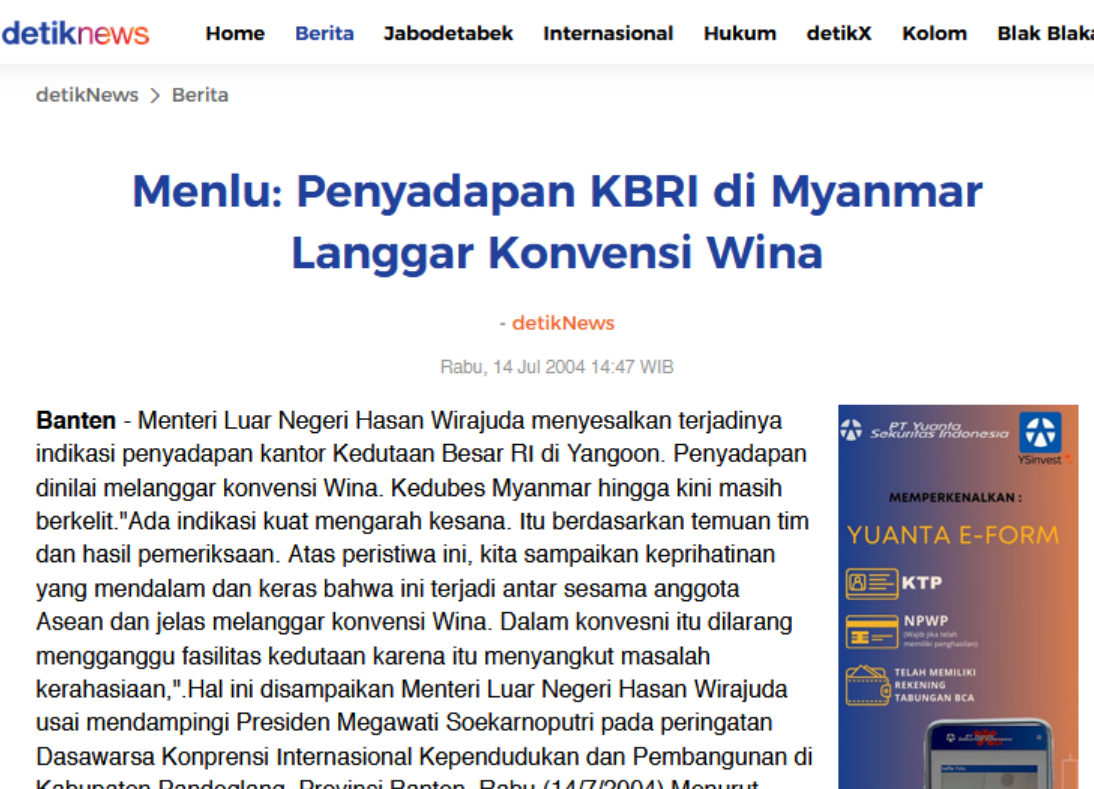
\includegraphics[width=119.70mm,height=216.81mm]{../../images/llm/page_017_img_01.png}%
\end{textblock*}

\end{document}
